\documentclass[]{report}
\usepackage{amsmath}
\usepackage{graphicx}
\usepackage[numbers,sort]{natbib}
\usepackage{array}
%\usepackage{todonotes}
% Title Page
\title{Convolutional Neural Networks and their Potential Hardware Acceleration}
\author{Magnus Halvorsen}


\begin{document}
%\maketitle
%This is the Titlepage
%%=========================================
\thispagestyle{empty}

\includegraphics[scale=0.3]{Figures/ntnu}
\mbox{}\\[6pc]
\begin{center}
\Large{TDT4900 Computer Science, Master thesis}\\[1pc]
\Huge{FANCY TITLE }\\[2pc]

\Large{Magnus Halvorsen}\\[1pc]
\large{Spring 2015}\\[2pc]


Department of Computer and Information Science\\
Norwegian University of Science and Technology
\end{center}
\vfill

\noindent Supervisor 1: Donn Alexander Morrison

\noindent Supervisor 2: Yaman Umuroglu
\setcounter{page}{0}
\pagenumbering{roman}
\section*{Assignment}

\textbf{Candidate name:} Magnus Halvorsen \\ \hfil \\ \hfil
\textbf{Assignment title:} Energy efficient machine learning algorithms in hardware \\ \hfil \\ \hfil
\textbf{Supervisors:} Donn Morrison and Yaman Umuroglu \\ \hfil \\ \hfil
\textbf{Assignment text:} \\ \hfil
The aim of this project is to explore the implementation of machine learning algorithms in hardware (e.g., FPGA) with the intention of improving energy efficiency over traditional implementation in software. The algorithm should be modularly developed so that it can be potentially used as an accelerator tile within a multi-core heterogeneous computing platform such as SHMAC. \\ \hfil \\ \hfil
For a given algorithm, e.g., a deep neural network, the student will:

\begin{enumerate}
	
	\item Explore the feasibility and expected efficiency gain over a general-purpose CPU (e.g., is there a need?)
	
	\item A literature survey on related techniques, hardware implementations, etc.
	
	\item Allocation of components between hardware and software (e.g., according to a HW/SW co-design methodology)
	
	\item If time permits, adapting the module for use as a SHMAC accelerator tile
	
\end{enumerate}
\begin{abstract}
The breakdown of Moore's Law and the effects of Dark Silicon have forced a paradigm shift from performance-centric serial computation to energy-efficient parallel computation. This has sparked an interest in heterogeneous computing, where the processor contains different cores and accelerators that are specialized for certain tasks. The SHMAC project aims to provide a research
platform for heterogeneous systems research. This has led to a need of exploring what kind of applications are worth accelerating. 

One such application is the Convolutional Neural Network algorithm, which is a state of the art technique for recognizing objects in images and sound. In this report we will explore the potential gains of creating a hardware accelerator for such a network. We will introduce the mathematical fundamentals behind the algorithm, provide an overview of the most recent suggested hardware architectures, and present our architecture, Imagezor.

\end{abstract}
\tableofcontents
\listoffigures
\listoftables
\setcounter{page}{0}
\pagenumbering{arabic}
\chapter{Introduction}


The aim of this project is to explore the implementation of machine learning algorithms in hardware (e.g., FPGA) with the intention of improving energy efficiency over traditional implementation in software. The algorithm should be modularly developed so that it can be potentially used as an accelerator tile within a multi-core heterogeneous computing platform such as SHMAC.

For a given algorithm, e.g., a deep neural network, the student will:

\begin{itemize}
	
	\item Explore the feasibility and expected efficiency gain over a general-purpose CPU (e.g., is there a need?)
	
	\item A literature survey on related techniques, hardware implementations, etc.
	
	\item Allocation of components between hardware and software (e.g., according to a HW/SW co-design methodology)
	
	\item If time permits, adapting the module for use as a SHMAC accelerator tile
	
\end{itemize}


big data

most efficient way of recognize objects in images

internet of things

energy effiencey
\chapter{Background}

In this chapter we will go through the fundamental mathematics and concepts behind the \textit{Convolutional Neural Network} (CNN) model, in order to be able to recognize which operations that can be hardware-accelerated. It gives a basic introduction to both general neural networks and \textit{CNNs}. The last section gives an overview of the research and state-of-the-art hardware implementations of CNNs. 

\section{Artificial Neural Networks}

An \textit{Artificial Neural Network} (ANN) is a computational model that is used for machine learning and pattern recognition. The name and basic concept is inspired by how the animal brain uses a network of neurons to recognize and classify objects. 

An ANN can intuitively be viewed as a probabilistic classifier. Depending on the input data it will output the probability that the data belongs to a certain \textit{class} (e.g. an object in an image or an investment decision). As the brain it can be trained to recognize different classes by being provided a set of labeled training data, e.g. a set of faces and a set of non-faces. It can then learn to decide whether a image contains a face or not. This is called supervised learning. The network can also be trained unsupervised, by providing it with a set of unlabeled images. It will then learn to recognize a set of classes, but will be unable to label them.  

The topology of an ANN is a number of layers containing a set of so-called neurons. A neuron takes as in a set of inputs (e.g. image pixels), where each input is associated with a respective weight. The input and the weight are then multiplied and summed, and the result is used to calculate a non-linear activation function. More formally a neuron is defined as follows: 

\begin{equation*}
Input: \{x_1, x_2,\dots, x_n\} = \mathbf{x} 
\end{equation*}

\begin{equation*}
Output: f(\mathbf{w^{T}x)} = f(\sum_{i=1}^{n}w_i x_i + b)
\end{equation*}

\textbf{w} is the connection weights, b is the neuron bias and \textit{f(...)} is the activation function. \textit{f(...)} tends to be either:

\begin{equation*}
Sigmoid: f(z) = \frac{1}{1 - e^{-z}}, \in [0,1]
\end{equation*}

or 

\begin{equation*}
Hyperbolic tagent: f(z) = tanh(z) = \frac{e^z - e^{-z}}{e^z + e^{-z}}, \in [-1,1]
\end{equation*}

An ANN consist of $ n_l $ layers, each containing a set of neurons. The first layer is \textit{the input layer}, and the last layer is \textit{the output layer}. The layers in between are called \textit{the hidden layers}. Each layer uses the previous layer output as input. The input layer is provided with the initial input and calculates its activation functions (one for each neuron). The result is propagated to the first hidden layer, and continues up until it reaches the output layer - which provides the final output. This is known as a \textit{feedforward neural network.}

The network takes in two parameters, $ (\mathbf{W, b}) = (\mathbf{w^{(1)}, b^{(1)}}, 
\mathbf{w^{(2)}, b^{(2)}}, \dots , 
\mathbf{w^{(n_l)}, b^{(n_l)}}) $. Then $ w_{ij}^l $ denotes the weight between neuron j in layer l, and neuron i in layer l+1. $ b_i^l $ denotes the bias associated with neuron i in layer l+1.

During the training of the network it is the parameters $ (\mathbf{W, b}) $ that are altered in order to adapt the network to the training data. This is done by providing the network with a set of training examples, where we provide an input and an expected output. We then use a cost function to compute the error of the actual output. Our goal is to minimize the cost function, so the actual output is as close as possible to the expected output. This can be done by a technique called gradient decent. 

Let the cost function for a single training example $(x,y)$ be defined as follows:

\begin{equation*}
	Cost(\mathbf{w},b; x, y) = \frac{1}{2}(h_{\mathbf{w},b}(x) - y)^2
\end{equation*}

Where $ x $ is the input, $ h_{\mathbf{w},b}(x) $ is the actual output of the ANN and \textit{y} is the correct output.
Then the cost function for \textit{m} training examples $ ((x^{1}, y^{1}), (x^{2}, y^{2}), \dots, (x^{m}, y^{m})) $ is:

\begin{equation*}
	Cost(\mathbf{w},b) = \frac{1}{m}\sum_{i=1}^{m}Cost(\mathbf{w},b;x^{(i)},y^{(i)}) + \frac{\lambda}{2}
	\sum_{l=1}^{n_l-1}\sum_{i=1}^{s_l}\sum_{j=1}^{s_l+1}
	(\mathbf{w}_{ji}^{l})^2
\end{equation*}
 
The first term is simply the average sum-of-squares error term. The second term is the \textit{text}regularization term, or \textit{weight decay term}, which tends to reduce \textit{overfitting}.

Based on this we can use \textit{gradient decent} to compute how we should alter the weights in order to reduce the cost function. One iteration of gradient descent updates \textbf{w} and \textit{b} as follows:

\begin{equation*}
	\mathbf{w}_{ij}^{(l)} = \mathbf{w}_{ij}^{(l)} - \alpha\frac{\partial}{\partial\mathbf{w}_{ij}^{(l)} }Cost(\mathbf{w},b)
\end{equation*}

\begin{equation*}
	\mathbf{b}_{i}^{(l)} = \mathbf{b}_{i}^{(l)} - \alpha\frac{\partial}{\partial\mathbf{b}_{i}^{(l)} }Cost(\mathbf{w},b)
\end{equation*}

Where $ \alpha $ is the learning rate, which is a predetermined constant. Note that this would only make us able to compute the gradient for the output layer. In order to perform gradient decent on the hidden layers, we need to propagate the error from the output layer backwards, to the hidden layers. For this we use the \textit{backpropagation algorithm}. Let $ o_i^{(l)} $ denote the output of the $i$th neuron in layer $l$, and $z_k^{(l)}$ is the weighted sum of the inputs plus the bias for the $k$th neuron in layer l. Then the \textit{backpropagation algorithm} can be formalized as follows: 

\begin{enumerate}
	\item Perform a feedforward pass, computing the output of every layer.
	\item For each output neuron k in the output layer, compute: 
	\begin{equation*}
		\delta_k = \frac{\partial}{\partial z_{k}^{(n_l)} }Cost(\mathbf{w},b; x, y) = -o_k^{n_l}(1-o_k^{n_l})(y_k-o_k^{n_l})
	\end{equation*} 
	\item For each hidden layer $ l = n_l - 1, n_l - 2,\dots, 2 $ compute: 
	\begin{equation*}
		\delta_i^{l} = o_i^l(1-o_i^l)\sum_{j=1}^{s_{l+1}} w_{ij}^l \delta_j^{l+1} 
	\end{equation*}
	\item Compute the partial derivative for each weight and bias:
	\begin{equation*}
		\frac{\partial}{\partial\mathbf{w}_{ij}^{(l)} }Cost(\mathbf{w},b; x, y) = o_j^{(l)}\delta_i^{(l+1)}
	\end{equation*}
	
	\begin{equation*}
		\frac{\partial}{\partial\mathbf{b}_{i}^{(l)} }Cost(\mathbf{w},b; x, y) = \delta_i^{(l+1)}
	\end{equation*}
\end{enumerate}
	
Now, combining \textit{gradient decent} and the \textit{backpropagation algorithm} we can describe an algorithm to train our network: 

\begin{enumerate}
	\item Initialize the weights $ \mathbf{w}^{(l)} $ and $ b^{l} $ for all \textit{l}.
	\item Do steps 3 to 5 until the $ Cost(\mathbf{w}, b; x, y) $ function is low enough or converges. This is referred to as an \textit{epoch}.
	\item Set $ \Delta\mathbf{w}^{(l)} := 0 $ and $ \Delta b^{(l)} := 0 $ for all \textit{l}.
	\item For i = 1 to m,
		\begin{enumerate}
			\item Use the backpropagation algorithm to compute $ \nabla_\mathbf{w^{(l)}}Cost(\mathbf{w}, b;x,y) $ and $ \nabla_b^{(l)}Cost(\mathbf{w}, b;x,y) $.
			\item  Set $ \Delta\mathbf{w}^{(l)} := \Delta\mathbf{w}^{(l)} + \nabla_\mathbf{w^{(l)}}Cost(\mathbf{w}, b;x,y) $. 
			\item  Set $ \Delta b^{(l)} := \Delta b^{(l)} + \nabla_{b^{(l)}}Cost(\mathbf{w}, b;x,y) $. 
		\end{enumerate}
	\item Update the parameters:
		\begin{equation*}
			\mathbf{w}^{(l)} = \mathbf{w}^{(l)} - \alpha[(\frac{1}{m}\Delta\mathbf{w}^{(l)}) + \lambda\mathbf{w}^{(l)}]
		\end{equation*}
		
		\begin{equation*}
			b^{(l)} = b^{(l)} - \alpha[\frac{1}{m}\Delta b^{(l)}]
		\end{equation*}
\end{enumerate}

\section{Convolutional Neural Network}

\textit{Convolutional Neural Network}\cite{LeCun1998} (CNN) is a variation of the \textit{Artificial Neural Network} model, which is mainly used for object recognition in images. It addresses three major problems the standard ANN model faces when it comes to object recognition. First, even small images contains a large amount of pixels/inputs, e.g. a $ 32 \times 32 $ image contains 1024 pixels/inputs. A fully connected network with 100 hidden units would then end up with $ 1024 \times 100 $ weights that needs to be calculated in the first layer! Making it computationally infeasible and not scalable. Second, objects of the same class are seldom exactly alike, something the network has to take into consideration. While possible, the network would have to be very large, would probably contain several neurons with similar weight vectors positioned at different places in the network, and would require a very large number of training samples. Third, a fully connected ANN does not take into consideration the topology of the input. An image has a strong 2D spatial locality correlation, which makes it possible to combine low-order features (edges, end-points etc.) into higher-order features.  


\begin{figure}[h!]
  \centering
      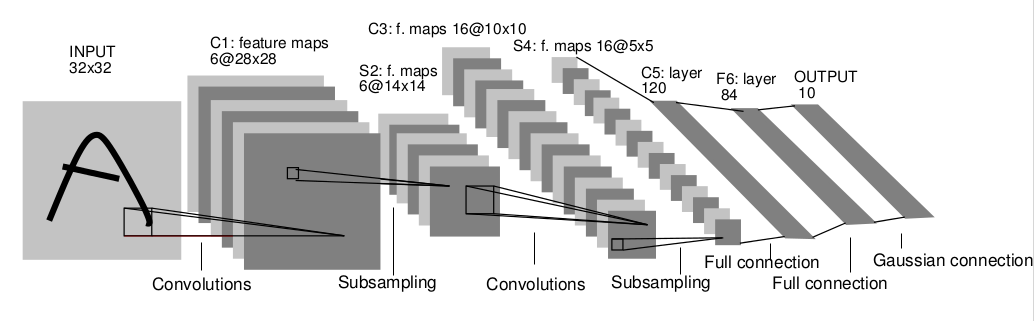
\includegraphics[width=1.0\textwidth]{Figures/Background/convnet}
  \caption{An example CNN, the LeNet-5\cite{LeCun1998}. }
\end{figure}

The CNN model adds two additional types of layers, in addition to the standard ANN layers: a convolution layer and a pooling/subsampling layer.

The idea behind the two new layers is to exploit the strong 2D local structure of images, i.e. pixels close to each other are highly correlated. By using local correlation one can extract and combine small local features (e.g. edges, corners, points) into higher-order features (e.g. nose, mouths, forehead), which can in the end be recognized as an object (e.g. a face). 

Intuitively, the convolution layer performs the feature extraction by applying a filter (kernel) on the whole image, and puts the result in a corresponding feature map. E.g. if the filter extracts vertical edges, only the vertical edges from the original image would remain in the resulting feature map. Thus you can extract different features by having several feature maps with different filters.  

Formally we can define a 2D convolution as follows. Let $ x_{ij} $ denote a value of the input matrix, $ w_{mn} $ denotes a value in a $ k \times k $ kernel matrix, and $ o_{ij} $ denotes a value of the output matrix. Then we get the following formula:

\begin{equation*}
o_{ij} = \sum_{m=1}^{k}\sum_{n=1}^{k} x_{i+m, j+n}w_{mn}
\end{equation*}


Once you have detected a feature, the exact position become less important. For example, the distance between the mouth and the eyes tend to vary between persons. So in order to make the \textit{CNN} not too sensitive to the relative placement of features, the accuracy of the feature map needs to be reduced. This can be done by partitioning the feature map into equal sized non-overlapping matrices, and then perform a pooling operation on each respective matrix. There are two types of pooling operations which are used for CNNs: 

\begin{itemize}
	\item \textit{Max-pooling} extracts the maximum value of the matrix.
	\item \textit{Average-pooling} extracts the average value of all the elements in the matrix.
\end{itemize}

In our solution we have opted for the max-pooling model, since its implementation is both easier and requires less resources. Formally it can be defined as:

\begin{equation*}
o_{ij} = max(x_{})
\end{equation*}

\begin{figure}[h!]
  \centering
      
\includegraphics[width=1.0\textwidth]{Figures/Background/Convolution-Maxpooling}
  \caption{Illustration of the convolution and subsampling/max-pool layers. First the input image is convolved with the kernel, then the resulting feature map is subsampled/max-pooled.}
\end{figure}

\section{Related Work}
The mathematical fundamentals for Convolutional Neural Networks was introduced as early as in the 1980s by Kunihiko Fukushima\cite{Fukushima1980}\cite{Fukushima1982}, in form of the \textit{neocognitron} model. The model was later improved in 1998 by  Yann LeCun, Léon Bottou, Yoshua Bengio, and Patrick Haffner - who introduced the \textit{Convolutional Neural Network} model. In 2003 the model was simplified by Patrice Simard, David Steinkraus, and John C. Platt \cite{Simard2000}, in an attempt to make it easier to implement. The paper also mentions two of the main issues with CNNs, size of the training set and time spent training. In order to achieve high enough accuracy a CNN requires thousands of training samples, which needs to be labeled. Processing all of these samples and fine-tuning the networks takes a great amount of processing power, causing training to take days or weeks. These issues are the ones that caused CNNs not to gain popularity before mid-2000. The rise of the Internet, digital cameras, and Big Data have provided us with vast amounts of images which can be used for training, and improvement in the speed and sophistication of computer hardware have reduced the training time from days/weeks to hours. E.g. \cite{Cires2003} purposes a GPU implementations which reduced the epoch training time from 35 hours to 35 minutes. 

In recent years CNNs have won several pattern recognition contests 


In \cite{Farabet2009} a CNN was implemented on a Virtex-4 SX35 FPGA from Xilinx. In this implementation all the fundamental computations was hard-wired, and controlled by a 32bit soft processor using macro-instructions. Training was done offline, and a representation of the network was provided to the soft processor. With this implementation they were able to process a $ 512 \times 384 $ grayscale image in 100\textit{ms}, i.e. 10 frames per second. 









\chapter{Related Work} \label{chap_related_work}

This section will give an overview of the current state of research on Convolutional Neural Networks. 

\section{Convolutional Neural Networks}
The mathematical fundamentals for Convolutional Neural Networks was introduced as early as in the 1980s by Kunihiko Fukushima\cite{Fukushima1980}\cite{Fukushima1982}, in form of the \textit{neocognitron} model. The model was later improved in 1998 by  Yann LeCun, Léon Bottou, Yoshua Bengio, and Patrick Haffner - who introduced the \textit{Convolutional Neural Network} model. In 2003 the model was simplified by Patrice Simard, David Steinkraus, and John C. Platt \cite{Simard2000}, in an attempt to make it easier to implement. The paper also mentions two of the main issues with CNNs: the size of the training set and the time spent training. In order to achieve high enough accuracy a CNN requires thousands of training samples, which needs to be labeled. Processing all of these samples and fine-tuning the networks takes a great amount of processing power, causing training to take days or weeks. These issues are the ones that caused CNNs not to gain popularity before mid-2000. The rise of the Internet, digital cameras, and Big Data have provided us with vast amounts of images which can be used for training. Improvements in the speed and sophistication of computer hardware have reduced the training time from days/weeks to hours. E.g. \cite{Cires2003} purposes a GPU implementations which reduced the epoch (see Section \ref{sec_ann_training}) training time from 35 hours to 35 minutes. This demonstrates that highly parallel hardware vastly increases the effiency of neural networks compared to CPUs. 

These recent advancements have renewed the interest in neural networks, and increased the research done on the field. As a result CNNs have become a leading model within pattern recognition for computer vision. This can be illustrated by the fact that CNNs implementations have won several pattern recognition contests in the period 2009-2012, including IJCNN 2011 Traffic Sign Recognition Competition\cite{Ciresan2012} and the ISBI 2012 Segmentation of Neuronal Structures in Electron Microscopy Stacks challenge\cite{DanC.Ciresan2012}.


\section{Convolutional Neural Network in Hardware} \label{sec_related_work_cnn}

There have been several proposed hardware architectures during the last decade, and below we will describe the more recent and relevant architectures. If the reader is interested in even older implementations, one can refer to \cite{Benkrid2002}  \cite{Cardells-Tormo2005} \cite{Hui2007} \cite{Savich2007} \cite{Girones2005}.

In \cite{Farabet2009} a CNN was implemented on a Virtex-4 SX35 FPGA from Xilinx. In this implementation all the fundamental operations were accelerated by a special-made ALU, and controlled by a 32~bit soft processor using macro instructions. That is, they created macro instructions for convolution, non-linear function, subsampling/pool and dot product between values at identical locations in multiple 2D planes and a vector. Training was done offline, and a representation of the network was provided to the soft processor. With this implementation they were able to process a $ 512 \times 384 $ grayscale image in 100\textit{ms}, i.e. 10 frames per second. The design was intented for use in low power embedded vision  systems, e.g. robots, and the whole curcuit board used less than 15 W.

Farabet and LeCun later improved the mentioned architecture in \cite{Farabet2010}. In this design they added multiple parallel vector processing units and allowed individual
streams of data to operate within processing blocks. They were able to achieve 30 frames per second using 15 W. In addition they predicted a planned ASIC implementation of the system would increase the processing speed and reduce the power to 1 W. 


In \cite{Chakradhar2010} they explore how they can exploit the different the parallel nature of CNNs. They introduce types of parallelism found in CNNs, \textit{inter-output} and \textit{intra-output}. The first one comes from the observation that each feature map and the corresponding subsampling/pooling computation can be done in parallel. This is easily seen in the first layer. The second one refers to that the convolution of several inputs are combined to produce one feature map (see Figure \ref{fig_visual_conv_ss_mp}), where the individual convolutions can be done in parallel. This one is present in all of the convolution layers after the first layer. They exploit these observations by purposing a dynamically configurable coprocessor on a FPGA, which can switch between computing several different feature maps in parallel and processing several inputs to compute one feature map. By doing this they are able to fully utilize the parallel nature of a CNN and reduce the intermediate storage on the FPGA. Using a Virtex 5 SX240T FPGA with 1024 multiply-accumulate units they were able to outperform  a 2.3 GHz quad-core, dual socket Intel Xeon, and a 1.35 GHz C870 GPU by 4x to 8x. 

\cite{Paper} presents an architecture they named the \textit{nn-X}. For the implementation they used a Xilinx ZC706 platform, containing a Kintex-7 FPGA and two ARM Cortex-A9. They made acceleration units for the convolution and subsampling/pooling layers on the FPGA, while the fully-connected layers was processed by the ARM processors. [REVWRITE]This implementation seems to be the fastest of all the purposed FPGA implementations to date, able to perform up to 227 G-ops/s. In addition it seems to be the most energy efficient across all platforms, by being able to perform 25 G-ops/s-Watt. In the paper they compared it to a Intel i7-3720QM and a NVIDIA’s GTX 780 GPU, where it was shown that it was up to 20x more power efficient. This makes a strong case for hardware acceleration of CNNs in applications designed for energy efficiency. 

\cite{INSERT_PAPER} focuses one the challenges of memory bandwidth related to deep convolutional neural networks. They argue that while accelerators are fast, slow memory makes it difficult to saturate the accelerators with enough data. To combat this they purpose a memory access optimized routcing scheme, where they try do reduce the number of times a input map has to be transfered from memory to the accelerator. A crucial point here is that in general the output map is the sum of several convoluted input maps. Thus if a accelerator is only able to compute one output map at a time, the input maps have to be transfered to the accelerator several times. This architecture suggested reduces the amount of such transfers by having a DMA for every two accelerator, and making the DMA transfer the same data to both of its accelerators. The accelerators will either produce an intermediate results or a complete output map, depending on how many iterations it has run. There is a total if eight accelerators, four which used to combine intermediate results into complete output maps, and four to compute intermediate results. Using this memeory scheme they were able to decrease the memory access by 2x and increase the hardware utilization by 2x. 

Hardware acceleration of CNNs have also gained popularity within the data center field. The Internet and Big Data have made it viable to have servers that performs image classification, image recognition and natural language processing, using CNNs. Since the main expense of data centers are power usage, using specialized hardware accelerators that provides good performance at low power have gained increased popularity. A recent example is Microsoft which have experimented on using accelerators for CNNs in their data centers, which is described in \cite{Microsoft_paper}. In the paper they present a rather big architecture compared to the previous papers mentioned, which fit into a Stratix V D5 FPGA. The previous mentioned architectures generally contained accelerators that computed parts of the network and needed to be controlled by software through macro instructions. Something that can cause a lot of off-chip traffic. In contrast, this architecture is able to reduce software involvement and off-chip traffic by using an on-chip re-distribution network module, which reloads processed data back into the accelerator. The cost of reducing off-chip traffic this way causes the architecture to consume a larger amount of hardware resources, which is the reason they are using such a big FPGA as the Stratix V D5. It would thus not be viable for mobile application with an restricted amount of hardware resources, but suits servers well. The result is a 3x improvement from the previous best implementation of a Virtex 7, 134 images/s compared to 46 images/s. The system is still slower than a GPU implementation on a Tesla K40, which are able to process 500-824 images/s, but is almost twice as energy efficient. The FPGA implementation uses 25 W, while the Tesla K40 runs at 235 W. 


\chapter{Method}

My special method. 

\section{Architecture}

\subsection {Convolution layer}

A convolution layer takes \textit{n} images as input, $ I_1, I_2, \dots, I_n $, and produces \textit{m} intermediate outputs, $O_1, O_2, \dots, O_m $. It also contains \textit{m} kernels, $ K_1, K_2, \dots, K_m $. Each kernel $ K_i $ is convolved with all the input images, and each respective pixel from each convolution is then summed, added a bias to, and sent through a non-linear function. Afterwards the resulting matrix is subsampled/max-pooled, where it is divided into $ k \times k $ non-overlapping neighborhoods, from which the maximum value is extracted. The result of the max-pool operation is provides the output image $ O_i $. 
In the first layer of the network there is only one input image (i.e. $ n = 1 $), thus no summation is needed. 

The overall architecture of the convolution layer is separated into four modules. A convolution module, a summation buffer, a non-linear function module and a subsample/max-pool module.

\vspace*{1\baselineskip}
\textbf{The convolution module} is inspired by \cite{Farabet2009}. The input is a $ n \times n $ image \textit{I}, and the output is a $ (n-k+1) \times (n-k+1) $ convolved image \textit{C}, using a $ k \times k $ kernel \textit{K}. Every clock cycle the module takes in a pixel as input, and after a certain delay it will output a processed pixel almost every cycle. Each pixel is inputted once, left to right, one row at a time. 

It consists of 2D grid of multiply and accumulate (MAC) units which represents the convolution kernel. Thus the grid dimension is equal to the kernel dimension. In every MAC unit there is a register that contains the respective kernel weight. In every clock cycle the MAC units multiply the input pixel with its weight, and then accumulates the result from the previous cycle of the MAC unit to the left. 

At the end of each row of MACs there is $ n - k $ shift registers. The result of the last MAC in each row is stored in the first shift register, and the first MAC in each row takes the value of the last shift register of the previous row as accumulation input. The exception being the absolute first and last MAC unit. Every clock cycle the values in the shift registers are shifted to the right. 
	
By providing this delay you only have to input each pixel once during the convolution. Generally every pixel is needed for $ k \times k $ convolution operations (the exception being the pixels close to the boarders of the image). Thus the shift registers are used to store the intermediate values of the convolutions until a pixel that is needed for the respective convolution operation is inputted. 

The delay these shift registers cause are the reason for the delay before valid output pixels are produced. Thus from when the convolution starts, the module will start outputting when $ k-1 $ rows of the image have been processed. And for every new image row, there will be a $ k-1 $ cycle delay before output is valid. This is demonstrated by the fact that the input image is a $ n \times n $ matrix, while the output matrix is a $ (n-k+1) \times (n-k+1) $ matrix. 

The speed of the convolution module is bounded by the number of pixels in the input image. 
 
\chapter{Results and Discussion} \label{chap_results}

This chapter will present the results from performance testing our purposed architecture. Section \ref{sec_results} will present the setup to our experiments and their respective results, while Section \ref{sec_discussion} will provide our analysis of the results. 

\section{Results} \label{sec_results}

\subsection{Hardware Resources}

The architecture described in Chapter \ref{architecture} was prototyped on an \textit{Avnet Zedboard}, containing a \textit{Xilinx Zyngq-7020 All Programmable System-On-Chip} (SoC). The SoC contains two ARM Cortex-A9 processors, and a Artix-7 FPGA. 

The main reason for choosing this system was that it contains four DMA channels, and 220 DSP slices, which should have allowed us to run four fully saturated accelerators in parallel. Unfortunately resource constraint for our architecture turned out to be \textit{look-up tables} (LUTs)

In this prototype we were only able to use one of the two ARM processors for controlling the accelerator(s) and processing the layers that were not accelerated. Preferably we should have used both for processing layer C5 and F6, but we were unable to do so due to time constraints. 

(Not done yet, will add more information on what hardware resources on the FPGA was used, and how this changes when adding more accelerators). 


\subsection{Performance}

In order to determine the execution speed and power efficiency of our system we have compared it to the ARM Cortex-A9 CPU on the Zedboard and an ASUS X550JK laptop with a Intel Core i7 4710HQ CPU. Both CPUs ran the pure software implementation of the CNN, while our system used a combination of hardware and software, as described in \ref{chap_method}. We ran our own system with three different configurations:

\begin{itemize}
	\item Accelerating layer C1 and S2. 
	\item Accelerating layer C1, S2, C3 and S4.
	\item Accelerating layer C1, S2, C3 and S4. In addition, the input images was preprocessed from 32-bit floating point to Q16:16 fixed point. Thus the input to the accelerator does not have to be converted during execution.
\end{itemize}

In order to determine the energy efficiency of the different systems we used the metric \textit{images/Watt}, i.e. number of images processed per Watt. Note that these images are $ 32 \times 32 $, and thus processing one image corresponds to 331104 multiply-and-accumulate operations. We also included a metric for measuring execution speed, using images/second. Despite power efficiency being the main focus of this assignment, execution speed can be interesting for several applications and is closely related to power usage. 

The measurements were done by timing the processing of 10 000 images from the MNIST dataset, while measuring the power consumation. 

Total board power was determined by measuring over pin 1 and 2 on J21 on the Zedboard during execution. With the FPGA programmed and the accelerator activated the board measured to 4.68 W, while the ARM processor alone measured to 4.32 W. We were unable to measure the power consumption of the laptop directly, and therefore used the power estimation provided by ASUS, being 120 W \cite{ASUS}.  

The results can be seen in Figure \ref{fig_results_all_layers}.

\begin{figure}[h!]
	\centering
	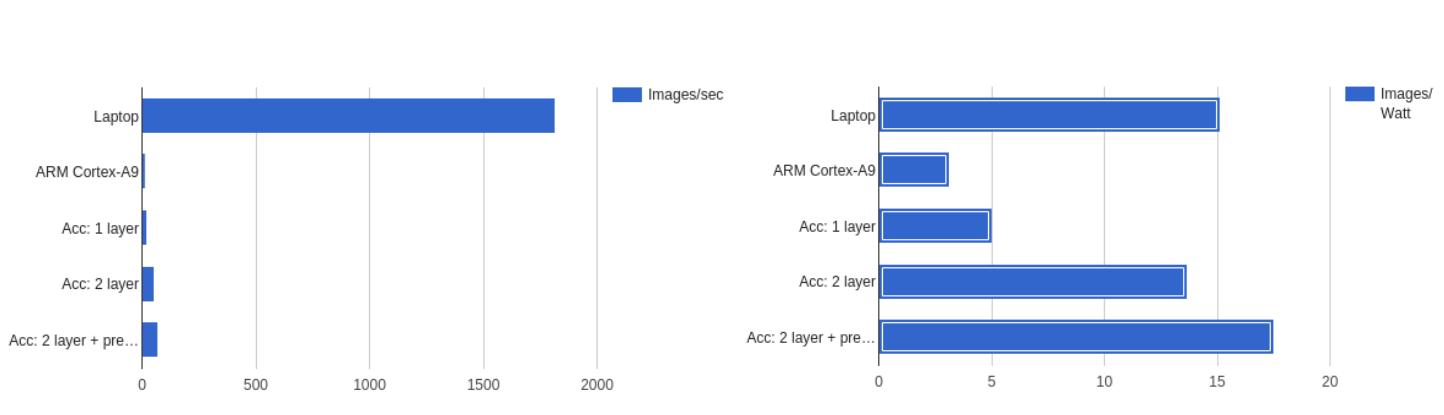
\includegraphics[width=1.0\textwidth]{Figures/Results/results_all_layers}
	\caption{The execution speed and power efficiency measured in number of images processed.}
	\label{fig_results_all_layers}
\end{figure}

We also decided to perform the same measurements when processing only the layers we have hardware accelerated, i.e. C1, S2, C3 and S4. This allowed us to compare the accelerator's performance more directly against the pure software implementations, since layer C5 and F6 shows to be the major bottleneck when processed on the ARM processor. The results are shown in Figure \ref{fig_results_accelerated_layers}.


\begin{figure}[h!]
	\centering
	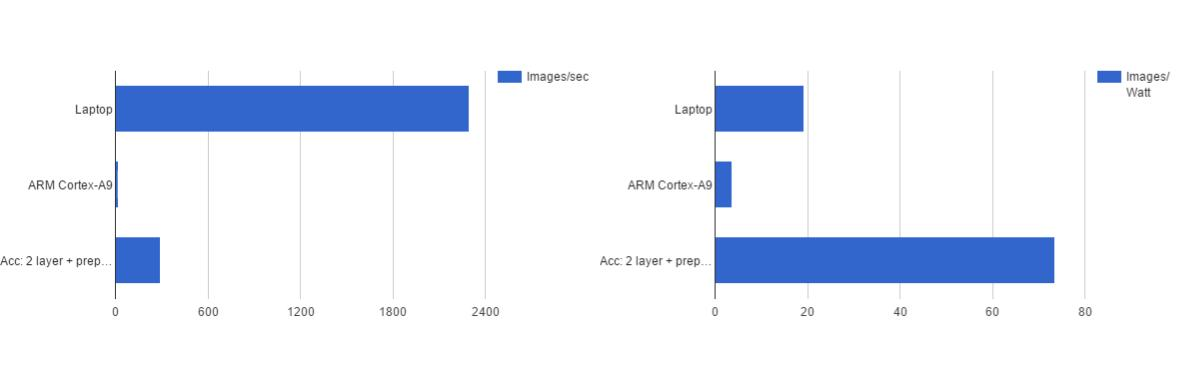
\includegraphics[width=1.0\textwidth]{Figures/Results/results_accelerated_layers}
	\caption{The execution speed and power efficiency measured in number of images processed.}
	\label{fig_results_accelerated_layers}
\end{figure}

\section{Discussion} \label{sec_discussion}

\subsection{Hardware Resources}

\subsection{Performance} 

As can be seen from the Figure \ref{fig_results_all_layers} the accelerator provides a significant boost to both execution and power performance compared to the ARM processor. Accelerating layer C1 and S2 provides a 1.6x speedup, while accelerating C1, S2, C3 and S4 provides a 4.3x speedup. Which is interesting since both layers computues about the same amount of connections (see Table \ref{tab_nofOps}), so why is the ARM processor able to compute C1 faster than C3? We deem that the most probable reason is the chache and memory accesses. In layer C1 the input image can be loaded into chache once and stay there for the duration of the processing of the layer. While in layer C3 there is a set of different input maps and kernels that is required to compute a single output map, thus reducing the ARM processors ability to utilize the cache. 

Figure \ref{fig_results_accelerated_layers} shows the performance when executing the layers that we have accelerated. Here we cleary see how much the accelerator outshines the ARM processor, with a 21x speedup. This also shows that the current bottleneck is now layer C5 and F6. In Section \ref{sec_what_to_accelerate} we deemed unlikely to be worth it to accelerate C5, but these results actually make a strong case for it. 

Compared to the ASUS X550JK our architecture is currently a lot slower, i.e. 26x slower. This is expected, since the laptop contains a state of the art CPU which is highly optimized for execution performance by Intel, while our accelerator is only a prototype. In addition, this network is a relatively small compared to the ones described in Chapter \ref{chap_related_work}, consequently leading to less parallelism to exploit. In addition when the input maps become to large to fit into cache, it is likley that the laptop's performance will drop. Thus with larger networks we predict that the difference between the execution time will decrease.

But while our accelerator performs worse in terms of execution speed it performs better in regard to power efficiency in some areas. When running all the layers, our system achieves 15.2 images/Watt while the laptop achieves 15.1 images/Watt, i.e. practice the same. But if we look at only the layers accelerated we see that our accelerator is 3x as power efficient. Based on this we believe that our systeme will outperform the CPU if the features mentioned in Chapter \ref{chap_related_work} are implemented.  

\chapter{Discussion and future work}

Should have had a GPU benchmark

Not able to fully exploit the parallelism of CNNS due to lack of hardware resources.

But easy to extend due to modular design

Havent been able to test the full design on FPGA
\chapter{Future work} \label{chap_future_work}

Developing a convolutional neural network hardware accelerator is a complex and time consuming task. There are thus several performance related improvements that we would wish to have implemented and tested, but sadly we ran out of time. In this chapter we will give an overview the planned, but unfinished, features we would wish to extend to our current architecture. The features are listed in a priority order, and we will give some indication of how much work is required to implement said features.


\begin{enumerate}                           


  \item \textbf{Improve the memory transfer and access scheme.}
    
    As we mentioned in Section \ref{sec_result_discussion}, the current memory access scheme is inefficient. This is because we transfer the same input maps multiple times to the accelerator, since different output maps require the same input maps. A better scheme would be to have two input buffers to the accelerator, one for input maps and one for weights/bias. One could then transfer all the input maps to the map buffer once, and let them reside there through the computations of the whole layer. The accelerator could then access the required input maps for the respective output map directly from that buffer. Thus would reduce off-chip trafic greatly, since the input maps are only transfered ones. It would require some extra control logic, so the accelerator acceses the corrent input maps in the buffer. 

	\item \textbf{Stream data through accelerator, instead of filling the buffer first.}
	
	Currently all the data required for computations are loaded into a buffer before it is processed by the accelerator. Changing it so that the data can be streamed directly into the accelerator would provide two potential benefits: 1) faster processing, since data can be processed while the DMA is transfering data to the accelerator, 2) reduced storage on chip, since we no longer need to store all the data in an input buffer. Should be fairly easy to extend the design for this, but due to time constraints, it was not implemented. 

  \item \textbf{Stay in hardware, instead of going back to software for next layer}
	
	The main reason \cite{Zhang2015} and \cite{Ovtcharov2015} achieved high performance was by reducing off-chip traffic. In the current state of our system, software has to be involved for every feature map to be computed, and data is being transfered back and forth between software and hardware several times. This is inefficient. Thus extending the system with logic that can redistrubute the output maps as new input maps without involving software could provide a substantial performance boost. But it will increase resource usage and development time, and will probably require a bigger board. Both the mentioned papers used FPGAs at the size of a Virtex 7. The mentioned improved memory scheme is a step in this directions. 
	
	\item \textbf{Explore ways to reduce the resource usage.}
	
	The primary focus of this project has been to get the prototype up and running, and little thought have gone to examine ways to minimize resource consumption. Currently we only have enough resources to fit two accelerators on the board. Thus if we wish to extend the design and/or run several accelerators in parallel, we either need to change to a bigger board or minimize the resource usage of our design. Any future work would do well to explore this area. 
	

	
	\item \textbf{More accelerators in parallel.}
	
	Currently we are only running two accelerators in parallel, which both have a respective DMA that moves their input and output data. The maximum DDR bandwidth is at about 3.2 GB/s, and each DMA has access to a \textit{high-performance} port which can  deliver up to 800 MB/s. This effectively means that we are exploiting half of the available DDR bandwidth. Given a big enough hardware platform or improvements to resource usage, as mentioned in the above point, this feature should be simple to implement. But before this can be exploited, the memory access scheme needs to be improved so the accelerators do not get starved. 
	
	
	
	\item \textbf{Hardware accelerate float to fixed.}
	
	Currently our system pre-processes the image and weights into fixed point before processing them. If this system were to be integrated into system using floating points it would be beneficial to do this transformation in hardware. Currently we are able to do fixed point to floating point in hardware using only one clock cycle, and thus we believe it should be possible to do the same for float to fixed. 

  \item Test with bigger images.

    
	\item \textbf{Training on hardware.}
	
\end{enumerate}

\chapter{Conclusion}

The goal of this project was to investigate the feasibility of implementing a hardware accelerator for a machine learning algorithm, which was chosen be a Convolutional Neural Network. In this report we have introduced the mathematical model behind CNNs, and shown how these can be trained in order to recognize objects in images. We have presented the Imagezor, an accelerator for CNNs which can be used even if hardware resources are sparse, with significant performance and energy efficiency gains. Based on this and the results from papers in Chapter \ref{chap_related_work}, we have shown that an accelerator will provide significant gains in both performance and energy efficiency.  


In the introduction we defined five tasks based on the original assignment text. The results from solving each of the tasks are presented below: \\ \hfil \\ \hfil
\textbf{Task 1. Choose a machine learning algorithm to investigate.} \\ \hfil \\ \hfil
The algorithm that was chosen was the Convolutional Neural Network algorithm. A lot of effort have been put into researching and understanding the algorithm, and the result from this effort can be found in the Chapter \ref{chap_background} and \ref{chap_related_work}. \\ \hfil \\ \hfil
\textbf{Task 2. Determine if a hardware accelerator will provide significant performance and energy-efficiency gains.}  \\ \hfil \\ \hfil
The papers presented in Chapter \ref{chap_related_work} makes a strong case for this. Many of them provides architectures that are at almost the sample level in performance as GPU implementations, while being up to 20x more energy efficient. In addition the results from simulating and comparing our design to a Intel Core i5 show significant performance and energy-efficiency gains. \\ \hfil \\ \hfil
\textbf{Task 3. Begin the development of a hardware accelerator for the chosen machine learning algorithm.}\\ \hfil \\ \hfil
Chapter \ref{architecture} presents our architecture Imagezor which can be used to accelerate the operations of a CNN. It has been shown to work in simulation, but have unfortunately not been tested on hardware. It has been designed in modular fashion, in order to make it easy as possible to adapt to a SHMAC tile. \\ \hfil \\ \hfil
\textbf{Task 4. Provide an overview of the state of the art of software and hardware implementations of CNNs.} \\ \hfil \\ \hfil
A literature survey of state of the art implementations have been presented in Chapter \ref{chap_related_work}.\\ \hfil \\ \hfil
\textbf{Task 5. Adapt the module to a SHMAC accelerator tile.} \\ \hfil \\ \hfil
As much effort went into researching CNNs, there was little time left for actual implementation. While an accelerator module was made, time did not permit it being extended to a SHMAC tile. \\ \hfil \\ \hfil




 
\bibliographystyle{unsrt}
\bibliography{myreferences.bib}


\end{document}          
